\documentclass[11pt,letterpaper]{article}
\usepackage[margin=0.82in,headheight=15pt]{geometry}
\usepackage[T1]{fontenc}
\usepackage{lmodern,amsmath,amssymb,mathtools,booktabs,array,graphicx}
\usepackage{xcolor,microtype,enumitem,fancyhdr}
\definecolor{navy}{HTML}{18384E}\definecolor{teal}{HTML}{137F8C}\definecolor{pale}{HTML}{EDF4F6}
\usepackage[colorlinks=true,linkcolor=navy,urlcolor=teal,citecolor=navy]{hyperref}
\hypersetup{pdftitle={Finite-momentum metric, radion and scalar response},pdfauthor={Prepared for Christopher Michael Baird with OpenAI Codex}}
\pagestyle{fancy}\fancyhf{}
\fancyhead[L]{\small\color{navy} MQGT--SCF / FINITE-MOMENTUM POLE TESTS}
\fancyhead[R]{\small 22 October 2026}
\fancyfoot[L]{\small Restricted classical operator; stated continuation}
\fancyfoot[R]{\small\thepage}
\setlength{\parindent}{0pt}\setlength{\parskip}{5pt}
\setlist{nosep,leftmargin=1.5em}\emergencystretch=2em
\widowpenalty=10000\clubpenalty=10000
\DeclareMathOperator{\Tr}{Tr}\DeclareMathOperator{\diag}{diag}
\newcommand{\dd}{\mathrm d}\newcommand{\Lam}{\Lambda}
\newcommand{\HH}{\mathcal H}\newcommand{\KK}{\mathcal K}\newcommand{\JJ}{\mathcal J}
\newcommand{\GE}{G^{\mathrm E}}\newcommand{\GJ}{G^{\mathrm J}}
\newcommand{\TimelikeTable}{\begin{tabular}{llrrrr}
\toprule $\epsilon$ & profile & $s_1$ & $s_2$ & $s_r$ & $s_{\rm extra}$\\\midrule
$0.01$ & $f_-$ & $0.009872633$ & $0.020017435$ & $0.656507988$ & $5.185494408$\\
$0.01$ & $f_+$ & $0.009872596$ & $0.020017355$ & $0.656500806$ & $5.184664332$\\
$0.0001$ & $f_-$ & $9.8394618\times10^{-5}$ & $2.0000177\times10^{-4}$ & $0.658115927$ & $5.185576700$\\
$0.0001$ & $f_+$ & $9.8360951\times10^{-5}$ & $1.9993330\times10^{-4}$ & $0.658108778$ & $5.184747238$\\
\bottomrule\end{tabular}}
\newcommand{\TachyonTable}{\begin{tabular}{llrr}
\toprule $\epsilon$ & profile & $z_T$ & $z_S$\\\midrule
$0.01$ & $f_-$ & $10.261011853$ & $10.902589419$\\
$0.01$ & $f_+$ & $10.260981092$ & $10.902556717$\\
$0.0001$ & $f_-$ & $10.253644490$ & $10.895573171$\\
$0.0001$ & $f_+$ & $10.253613710$ & $10.895540395$\\
\bottomrule\end{tabular}}
\newcommand{\CountTable}{\begin{tabular}{llrr}
\toprule $\epsilon$ & profile & tensor zeros & coupled zeros\\\midrule
$0.01$ & $f_-$ & 7 & 33\\
$0.01$ & $f_+$ & 9 & 37\\
$0.0001$ & $f_-$ & 7 & 33\\
$0.0001$ & $f_+$ & 9 & 37\\
\bottomrule\end{tabular}}
\newcommand{\ResidueTable}{\begin{tabular}{rrl}
\toprule $s=-z$ & $Z$ & residue sign\\\midrule
$-10.902589419$ & $-2.749610742$ & negative\\
$0.009872633$ & $0.993141487$ & positive\\
$0.020017435$ & $0.986123823$ & positive\\
$0.656507988$ & $0.631983970$ & positive\\
$5.185494408$ & $0.061470822$ & positive\\
\bottomrule\end{tabular}}
\newcommand{\CheckCount}{194}
\newcommand{\RealResidueError}{$4.4\times10^{-9}$}
\newcommand{\CutoffError}{$4.4\times10^{-15}$}
\newcommand{\QuadratureError}{$1.4\times10^{-14}$}
\newcommand{\PoleShift}{$7.7\times10^{-14}$}
\newcommand{\ComplexShift}{$1.1\times10^{-14}$}
\newcommand{\ComplexResidueError}{$5.9\times10^{-8}$}

\begin{document}
\thispagestyle{plain}
{\small\bfseries\color{teal} BAIRD / ZORAASI RESEARCH CONTINUATION}\par
{\LARGE\bfseries\color{navy} Finite-momentum metric, radion\\ and scalar response}\par
{\large Lorentzian pole tests and an obstruction in the minimal action}\par
\textbf{Prepared for Christopher Michael Baird with OpenAI Codex}\hfill 22 October 2026

\colorbox{pale}{\parbox{\dimexpr\linewidth-2\fboxsep\relax}{\textbf{Result.} The declared warped Dirac operator yields a metric-coupled two-point function with full external-momentum dependence. Its infrared limit reproduces the previous Einstein kinetic matrices. Under the explicitly tested continuation $z=p_E^2/\Lam^2=-s-i0$, the light neutral and radion-connected timelike poles have positive residues. However, the same retained action has a tensor tachyon, an additional neutral tachyon, negative residues at both, and non-real pole pairs. An analytic sign argument guarantees a positive-Euclidean-momentum tensor zero for the stated positive exponential profiles. This obstructs an unrestricted stable/unitary interpretation of this minimal action. It is not a complete compactification spectrum, a causal quantum propagator construction, or a proof against all possible completions of the program.}}

\section{Question, preserved input, and precise scope}

The radion note \cite{previous} derived positive nine-field Einstein kinetic matrices on four tuned fixtures, while explicitly withholding a physical-pole interpretation for the radion parameter near $0.91\Lam$. Its fixed-metric momentum diagnostic omitted the metric response needed to settle that question. This note derives the missing response, eliminates the metric trace only where legitimate, and searches the analytic two-point operator for poles and residues.

Inputs are pinned at commit \texttt{1bb152dfbd6bb1e02a3e841b6d73e338f8e5fabf}. We retain the parity-even full-Dirac action, four copied fermion blocks, unit dimensionless Yukawas, fixed monopole connection, positive ten-exponential profiles and lowest scalar harmonics. Both profiles $f_-$ and $f_+$ are evaluated at $\epsilon=10^{-2},10^{-4}$. Their scalar-mass counterterm is externally chosen; the flatness subtraction is separately selected per fixture. The inherited operator files and numerical inputs are copied unchanged with hashes in \texttt{provenance.json}.

Here ``finite momentum'' means exact external-momentum dependence at \emph{quadratic order in the declared fluctuations}. It does not mean an all-orders or quantum calculation. Internal sums are represented without a local curvature expansion but evaluated with finite fermion angular cutoffs. The physical pole tests concern the closed CP-even neutral radius/amplitude sector and the transverse-traceless four-dimensional metric. All nine fixed-metric scalar entries are supplied, but vector/axion constraints for charged and phase poles are outside this calculation.

\section{The quadratic operator at arbitrary external momentum}

\subsection{Internal background and the exact scalar kernel}

For $\dd s_6^2=g_{\mu\nu}(x)\dd x^\mu\dd x^\nu+r(x)^2\dd\Omega_2^2$, the classical spinor measure map of the predecessor gives
\begin{equation}
 D=D_g+\gamma_5\Lam B(q),\qquad q=(R,h_d,h_u,\ldots),\quad R=\Lam r.
\end{equation}
The three internal sectors have multiplicities $(n_q,n_\ell,n_0)=(12,4,12)$ and matrices $B_q=D_q/R+h_dS_d+h_uS_u$, $B_\ell=D_\ell/R+h_dS_\ell$, $B_0=D_0/R$. The cutoff remains fixed and
\begin{equation}
 S_{\rm sp}=\frac\kappa2\sum_a w_a\Tr e^{-aD^2/\Lam^2},\qquad a>0,\quad w_a>0.
\end{equation}
The symbol $a$ in a sum denotes a heat rate; $\mathsf a(z)$ below is a tensor form factor.

At a constant fixture diagonalize each $B$, with eigenvalues $b_i$, and define the Hermitian real-field tangents $T_A=\partial_A B$ and $A_A=\{B,T_A\}$. Let $\HH_{AB}=\partial_A\partial_B W$ be the total dimensionless potential Hessian, with all selected parameters fixed. The scalar kernel on a flat fixed Jordan metric is
\begin{align}
 \JJ_{AB}(z)&=\frac{\HH_{AB}}{4\pi^2}+\Delta_{AB}(z),\qquad z=p_E^2/\Lam^2,\label{eq:J}\\
 \Delta_{AB}(z)&=\frac1{8\pi^2}\sum_{a,s}w_an_s\sum_{ij}\int_0^1\!\dd t\,
 e^{-a[tb_i^2+(1-t)b_j^2]}\nonumber\\[-2pt]
 &\quad\times\left[z e^{-at(1-t)z}\,\operatorname{Re}(T_{A,ij}T_{B,ji})
 +(e^{-at(1-t)z}-1)\operatorname{Re}(A_{A,ij}A_{B,ji})\right].\label{eq:delta}
\end{align}
For complex $z$, the real part applies to the internal matrix product, \emph{not} to the momentum-dependent exponential. Thus the continued kernel is analytic. Charged tangents can connect distinct magnetic blocks; their corresponding two spectra are used in \eqref{eq:delta}. The full scalar assembly implements these transitions.

The zero-momentum term includes nonlinear radius contacts $B_{RR}$, the mass counterterm and the fixed subtraction. They are not to be discarded when constructing $\HH$. Their local momentum independence is why no additional contact appears in $\Delta(z)-\Delta(0)$. This kernel agrees with the predecessor's fixed-metric diagnostic; it is not yet the metric-coupled propagator.

\subsection{Resummed gravitational and mixed form factors}

Introduce two entire functions with removable values at the origin:
\begin{equation}
 F(x)=\int_0^1 e^{-xt(1-t)}\dd t,\qquad
 J(x)=\frac{1-F(x)}{x},\qquad F(0)=1,\quad J(0)=\frac16.\label{eq:FJ}
\end{equation}
At constant internal $B$, metric vertices are internal identities. Each internal mass therefore multiplies the external Dirac heat trace by $e^{-ab_i^2}$. Define
\begin{equation}
 H_a=\sum_s n_s\Tr e^{-aB_s^2},\qquad
 Q_{aA}=\sum_s n_s\Tr[e^{-aB_s^2}\{B_s,T_A\}],\qquad
 f=\sum_a\frac{w_aH_a}{48\pi^2a}>0.
\end{equation}
The exact quadratic metric and mixed functions are
\begin{align}
 \boxed{\mathsf a(z)=\sum_a\frac{w_aH_a}{16\pi^2a}
       [F(az)-4J(az)]},\label{eq:aa}\\
 \boxed{\mathsf b(z)=\sum_a\frac{w_aH_a}{16\pi^2a}
       [-\tfrac12F(az)+5J(az)]},\label{eq:bb}\\
 \boxed{c_A(z)=\sum_a\frac{w_aQ_{aA}}{16\pi^2}J(az)}.\label{eq:c}
\end{align}
In particular $\mathsf a(0)=\mathsf b(0)=f$ and $c_A(0)=-f_A/2$. Scalar amplitudes enter $H_a$ and $Q_{aA}$ at their finite fixture values; replacing them by unbroken values would lose the required mixing.

For derivation, specialize the standard nonlocal heat kernel \cite{CZ} to the Dirac endomorphism $U=\mathcal R/4+B^2+i\gamma^\mu\gamma_5\partial_\mu B$. The spin trace combines the curvature form factors into
\begin{align}
 C_{\rm Ric}(x)&=\frac{F(x)-1/3}{x}+4\frac{F(x)-1}{x^2},\\
 C_R(x)&=\frac{2-3F(x)}{12x}-\frac{F(x)-1}{2x^2}.
\end{align}
The limits are $C_{\rm Ric}(0)=-1/10$ and $C_R(0)=1/30$. Writing the Euclidean curvature terms as $\kappa[\beta(z)\mathcal R_{\mu\nu}\mathcal R^{\mu\nu}+\alpha_g(z)\mathcal R^2]$ gives
\begin{equation}
 (\beta,\alpha_g)=\frac1{32\pi^2}\sum_a w_aH_a(C_{\rm Ric},C_R)(az),\quad
 \mathsf a=f+2z\beta,\quad \mathsf b=f-4z(\beta+3\alpha_g).
\end{equation}
The mixed spin-trace combination is $4f_{RU}+2f_U=2J$, giving \eqref{eq:c}. A single mixed insertion selects diagonal elements of $\{B,T_A\}$; no assumption that all scalar matrices commute is used. Terms linear in the derivative endomorphism have vanishing spin trace in this mixed channel.

The local combination $\beta(0)+3\alpha_g(0)$ vanishes, but its momentum-dependent continuation does not. Dropping it at all momenta would incorrectly turn a local curvature-squared cancellation into a full propagator statement. The tensor result is consistent with known spectral-action momentum behavior \cite{KLV,ASZ}, with the zero-momentum potential contact treated as described next.

\subsection{Stationarity, metric constraints, and the bordered matrix}

The total potential includes the selected covariant potential terms. Its value and gradient vanish at each flat fixture, so all purely metric and mixed metric/potential contacts cancel. This step uses $W=W_A=0$, not merely a choice to omit a cosmological term. The parameters $\alpha$ and $c$ are held fixed in all derivatives. Neither term supplies independent momentum-dependent curvature vertices by assumption.

At nonzero momentum let $\theta_{\mu\nu}=\delta_{\mu\nu}-p_\mu p_\nu/p^2$, and
\begin{equation}
 P_0{}_{\mu\nu,\rho\sigma}=\frac13\theta_{\mu\nu}\theta_{\rho\sigma},\qquad
 P_2{}_{\mu\nu,\rho\sigma}=\frac12(\theta_{\mu\rho}\theta_{\nu\sigma}+\theta_{\mu\sigma}\theta_{\nu\rho})-P_0{}_{\mu\nu,\rho\sigma}.
\end{equation}
Use $\tau=\theta_{\mu\nu}h_{\mu\nu}/\sqrt3$ for the transverse trace and $h^{TT}$ for the spin-two field. Diffeomorphism gauge directions are omitted. With dimensionless coordinates $X=\Lam x$ and Fourier momentum $k=p_E/\Lam$, the quadratic action is
\begin{equation}
 \frac{S_E^{(2)}}{\kappa}=\frac12\int_k
 \left[h^{TT}(-k)K_2(z)h^{TT}(k)+
 \begin{pmatrix}\tau&\delta q^T\end{pmatrix}_{-k}
 \KK(z)\begin{pmatrix}\tau\\\delta q\end{pmatrix}_{k}\right],
\end{equation}
where $\int_k=\int\dd^4k/(2\pi)^4$, $z=k^2$, and
\begin{equation}
 \boxed{K_2(z)=\frac z4\mathsf a(z),\qquad
 \KK(z)=\begin{pmatrix}
 -z\mathsf b(z)/2&\sqrt3\,z c(z)^T\\
 \sqrt3\,z c(z)&\JJ(z)
 \end{pmatrix}.}\label{eq:K}
\end{equation}
For the pole search $q=(R,h_d,h_u)$, so this matrix is $4\times4$. CP and charge selection rules make these modes close with the metric at quadratic order in the declared family. Numerical transverse-projector contractions check the diffeomorphism Ward identities. The remaining scalar directions do not acquire a metric mixing term at this neutral real background.

Where $\mathsf b(z)\ne0$, eliminating $\tau$ gives
\begin{equation}
 \KK_{\rm red}(z)=\JJ(z)+\frac{6z}{\mathsf b(z)}c(z)c(z)^T,\qquad
 \KK_{\rm red}'(0)=\GJ+\frac{3}{2f}f_Af_B=\GE.\label{eq:Schur}
\end{equation}
This recovers the complete inherited infrared Einstein metric, including radion-amplitude mixing. At finite momentum it is a Schur complement, not a local Weyl transformation with a guessed kinetic coefficient.

The Schur expression is meromorphic even though the original quadratic kernels are entire. We therefore search
\begin{equation}
 D(z)=\det\begin{pmatrix}-\mathsf b(z)/2&\sqrt3\,c(z)^T\\
 \sqrt3\,z c(z)&\JJ(z)\end{pmatrix},\qquad \det\KK(z)=zD(z),\label{eq:entireD}
\end{equation}
and verify null vectors in the full matrix. The trivial metric $z$ factor is not a new propagating scalar. The negative Einstein-Hilbert conformal entry at the origin is the usual gravitational constraint; counting it alone as a scalar ghost would misread the gauge-invariant source exchange.

\section{Lorentzian continuation and pole diagnostics}

We test the direct continuation
\begin{equation}
 z=-s-i0,\qquad s=(\omega^2-|\mathbf k|^2)/\Lam^2.\label{eq:cont}
\end{equation}
The entire quadratic functions have an unambiguous analytic extension, but this alone does not construct a causal quantum propagator or justify rotating a path integral through sectors of exponential growth. An integration contour, asymptotic state space, reflection positivity and ultraviolet unitarity remain separate questions. No alternate prescription is chosen to remove inconvenient zeros.

A simple real zero $z_*$ gives $s_*=-z_*$. Negative $z_*$ is timelike with positive squared mass parameter; positive $z_*$ is tachyonic under \eqref{eq:cont}. At a full neutral null vector $v$, normalized by $v_q^T\GE(0)v_q=1$,
\begin{equation}
 \KK^{-1}(z)=\frac{v v^T}{(z-z_*)v^T\KK'(z_*)v}+O(1),\qquad
 Z=\frac1{v^T\KK'(z_*)v}.\label{eq:residue}
\end{equation}
The real sign is compared with a healthy Euclidean kernel $z+m^2$. For the tensor it is the sign of $1/K_2'(z_*)$; we also quote its ratio to the massless residue, $f/[4K_2'(z_*)]$. At non-real zeros the transpose bilinear still gives the residue matrix, but a positive/negative norm sign is not defined. Matrix-inverse limits independently check the residues.

\subsection{An analytic tensor obstruction}

Let $\nu_a=w_aH_a/(16\pi^2a)>0$. The tensor form factor obeys
\begin{equation}
 \mathsf a(0)=f>0,\qquad
 K_2(z)\underset{z\to+\infty}{\longrightarrow}
 -\sum_a\frac{w_aH_a}{32\pi^2a^2}<0.\label{eq:tensorobstruction}
\end{equation}
The second statement follows from $F(x)=2/x+4/x^2+O(x^{-3})$ in \eqref{eq:aa}. Since $K_2(z)>0$ for small positive $z$, continuity forces at least one nonzero positive-real zero. This argument applies to the specified positive finite exponential sum and convergent internal heat traces, not merely to a finite momentum polynomial. It uses the total flat-stationary subtraction; retaining an uncanceled off-shell potential contact would change the expansion point.

Conversely, for $s\ge0$ each term of the timelike tensor factor has the series
\begin{equation}
 F(-as)-4J(-as)=
 \sum_{n=0}^{\infty}\frac{n!}{(2n+1)!}\frac{2n+1}{2n+3}(as)^n>0.\label{eq:positive}
\end{equation}
Thus $\mathsf a(-s)$ has no real timelike zero. The ordinary massless tensor pole remains, with positive slope $f/4$. The sign argument does not enumerate all spacelike or complex zeros or establish their residue signs; those are tested numerically below. Additional independent gravitational operators would change the conclusion and are not included here.

\subsection{Real poles on the four fixtures}

Within $-20\le z\le20$, the neutral coupled search finds four timelike poles and one positive-$z$ pole on each fixture. The three low-lying timelike poles connect to the two light neutral modes and the radion of the preceding derivative truncation. The fourth lies above the cutoff. The reported timelike squared parameters $s=-z$ are:

\begin{center}\small\TimelikeTable\end{center}

The radion-connected value at $\epsilon=0.01$, $f_-$ changes from $0.829596301$ in the two-derivative calculation to $0.656507988$, a roughly $20.9\%$ reduction in the squared parameter. The corresponding mass parameter changes from $0.91082\Lam$ to about $0.81025\Lam$. This comparison is internal to the retained operator; the same fixture has the instability below, so it is not a stable-particle prediction. The small light shifts and positive residues do not remove that obstruction.

\begin{center}\small\TachyonTable\end{center}

Here $z_T,z_S>0$ imply $s_T,s_S<0$. Both real zeros have negative residue signs. For the representative minus fixture, the tensor relative residue is approximately $-3.42635$. The neutral real-pole residues, using the normalization in \eqref{eq:residue}, are:
\begin{center}\small\ResidueTable\end{center}

The tachyonic scales are above $\Lam$, where an infrared-only effective interpretation cannot support particle claims. They are nevertheless genuine zeros of the externally resummed quadratic action that was actually specified. If that minimal action is taken as an unrestricted directly continued theory, it fails these stability tests. Treating it only as an infrared effective action leaves the ultraviolet completion open; it does not prove that the omitted response is healthy.

The metric denominator $\mathsf b$ vanishes at $z\simeq-3.400860947$ on the representative fixture. This is \emph{not} a pole of the full coupled inverse: $D\simeq0.82203$ and the full matrix's smallest/largest singular-value ratio is about $0.519$. A search of the Schur denominator alone would report a spurious mode. The full bordered search avoids that error.

\subsection{Bounded complex-plane searches}

The argument-principle diagnostic counts zeros of the entire functions $\mathsf a(z)$ and $D(z)$ in the square $|\operatorname{Re}z|,|\operatorname{Im}z|\le20$. The known massless tensor factor $z$ is excluded, as is the trivial metric factor in \eqref{eq:entireD}. Counts agree under contour refinement:
\begin{center}\small\CountTable\end{center}

The different counts for the two matched profiles illustrate that infrared matching does not fix the complex response. These are bounded numerical counts, not a global classification or interval-certified theorem. On the representative $\epsilon=0.01$, $f_-$ fixture we separately isolate all three upper-half-plane tensor zeros and fourteen upper-half-plane coupled zeros, with their conjugates. Together with one and five real zeros respectively, they match the counts 7 and 33. The three tensor pairs begin at
\begin{equation}
 z\simeq-3.12718\pm4.11902i,\quad
 -3.77331\pm9.38205i,\quad
 -3.92396\pm14.51680i.
\end{equation}
The nearest coupled pairs include $-3.97523\pm4.08617i$ and the closely spaced pair locations $-2.11688\pm4.29363i$, $-2.12245\pm4.29509i$. The complete roots, null vectors or complex residue matrices, search cells and tolerances are in \texttt{results.json}. Other fixtures have real-pole results and refined enclosing contour counts, without an asserted individual enumeration of every non-real zero.

\begin{figure}[ht]
\centering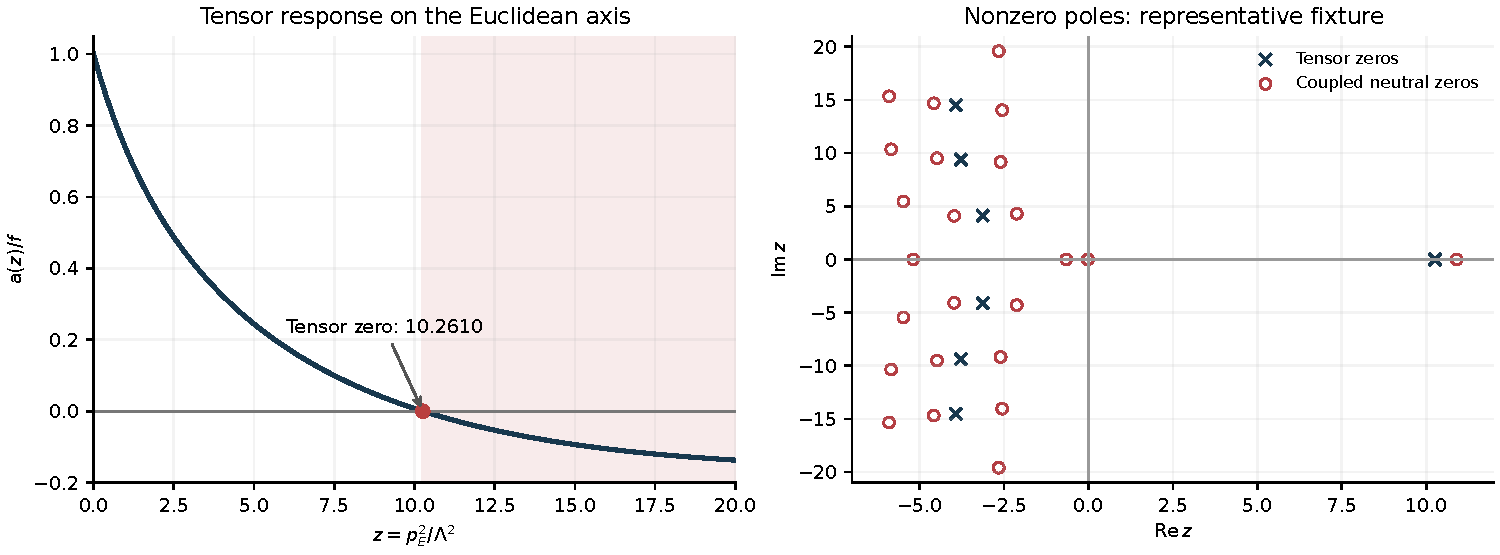
\includegraphics[width=\linewidth]{images/finite_momentum_poles.pdf}
\caption{Representative minus profile, $\epsilon=0.01$. Left: tensor factor $\mathsf a(z)/f$ on the positive Euclidean axis, crossing zero at $z\simeq10.2610$. Right: nonzero tensor and coupled neutral zeros inside the declared complex search square; conjugates are included. Closely spaced roots and the light poles near the origin overlap at this scale. The map is a bounded numerical result, not a physical particle spectrum.}
\end{figure}

Complex poles and negative-residue tachyons obstruct an ordinary positive spectral interpretation under the tested prescription. No claim is made that an unspecified nonstandard contour repairs them. Nor does this calculation prove the impossibility of every modified action or completion of the broader research program.

\section{Independent checks and reproduction}

The bundle contains \textbf{\CheckCount{} passing targeted checks}. They measure computational consistency, not independent physical predictions. The following tests connect the calculation to distinct derivations or numerical controls:
\begin{enumerate}
\item \textbf{Explicit Dirac vertices.} For a single constant internal eigenvalue, use $g_{\mu\nu}=e^{2\sigma}\delta_{\mu\nu}$ and the common-density operator $e^{-\sigma/2}D_{\rm flat}e^{-\sigma/2}+\gamma_5 b$. A second probe uses $g=\diag(1,e^{2\eta},e^{-2\eta},1)$, whose volume is fixed. Direct $4\times4$ gamma-matrix Duhamel vertices and shifted four-dimensional Gaussian integration check the conformal, scalar/mixed and tensor kernels without using curvature form factors. Three-point Hermite quadrature integrates the Gaussian polynomial moments exactly. Fifteen combinations of mass, heat rate and real/complex momentum agree within approximately $6\times10^{-16}$.
\item \textbf{Infrared and symmetry controls.} The old Jordan and Einstein matrices are recovered, including the mixed entries. All-nine-field assembly reproduces the inherited metric and the neutral finite-momentum block. Transverse projectors satisfy metric and mixed diffeomorphism contractions. The scalar/metric selection rule and complex-conjugation symmetry are checked.
\item \textbf{Derivatives and residues.} Analytic momentum derivatives agree with five-point finite differences. Full-operator null residuals are tested at each real pole, and matrix-inverse limits check real and representative complex residue matrices. The maximum relative residue-limit discrepancies are approximately \RealResidueError{} (real) and \ComplexResidueError{} (complex).
\item \textbf{Cutoffs and contours.} Increasing the fermion cutoff from 12 to 16 changes sampled normalized kernels by at most \CutoffError{} and real neutral pole positions by at most \PoleShift{}. Changing 64-point to 96-point quadrature changes sampled normalized kernels by at most \QuadratureError{}. Representative complex pole shifts under these controls are at most \ComplexShift{}. These observed differences are not error certificates. Enclosing counts are stable under contour refinement; adaptive subdivision resolves pairs missed by an initial multi-start search.
\end{enumerate}

The runner supplies full matrices, analytic derivatives, real pole residues, bounded complex counts and representative complex residues. It exits nonzero on failed checks. A writable extraction can be rerun after installing the recorded NumPy/SciPy dependencies; figure generation also uses Matplotlib. The final delivery record documents fresh-extraction reproduction, compilation, visual inspection and hashes. Byte identity is environment dependent.

\section{Assumptions and what remains unresolved}

These qualifications are part of the result. The bundle's \texttt{ASSUMPTIONS.md} gives the complete twelve-item statement, including the inherited axion and normalization assumptions.
\begin{enumerate}
\item \textbf{Restricted backgrounds.} The torsion-free warped round sphere, fixed monopole data, microscopic insertion, unit Yukawas and lowest scalar harmonics are specifications, not a proven unique or phenomenologically viable reduction. All external momenta are retained only at quadratic fluctuation order. Finite fermion angular cutoffs are not a complete bosonic truncation.
\item \textbf{Selected potential terms.} The mass counterterm and flatness subtraction remain chosen inputs, fixed in derivatives and minimally covariantized. They supply no extra curvature or derivative terms by assumption. Allowing such terms changes the operator; none is introduced to erase the observed poles. This is not a cosmological-constant solution.
\item \textbf{Continuation is conditional.} The direct continuation \eqref{eq:cont} defines the tested analytic functions. It does not prove a quantum Wick rotation, a causal contour, a well-posed nonlocal initial-value problem, positive spectral representation, reflection positivity or ultraviolet unitarity. The complex growth of heat form factors requires care. The real residue convention is stated explicitly; complex residues have no norm sign assigned.
\item \textbf{No stable vacuum claim.} Positive-residue timelike modes coexist with tachyonic and complex poles in the retained operator. The previous infrared tests remain valid within their derivative scope, but do not extend to an unrestricted stable minimal action. Above-cutoff pole positions are not measured particles. The radion-connected pole is still a conditional quadratic result, not a certified excitation of a complete stable theory.
\item \textbf{Omitted fields and stationarity.} Higher scalar harmonics, nonspherical internal metric modes, other gauge/bosonic fluctuations and their tadpoles have not been solved or integrated out. Their mixing can shift poles, and the inherited restricted stationary point need not be a stationary point in the full theory. No nonlinear stability, global minimality, uniqueness, vacuum lifetime or stable compactification is proved. The untuned runaway remains an inherited separate result.
\item \textbf{Gauge and axion boundary.} Physical pole searches use the CP-even neutral/metric and TT sectors. Charged and phase kernels require a full vector/axion constraint analysis for pole interpretation. The earlier potential-free axion with positive independent coefficient, pure-$X$ Stueckelberg coupling and no additional derivative mixing remains an assumption, with one physical phase massless. The anomaly polynomial, two-form reduction, axion potential and Stueckelberg scale remain unspecified.
\item \textbf{Numerical scope.} Real and complex domains are explicitly bounded. Refined contours and root residuals are not interval-certified counts, uniform tail bounds or global zero enumeration. Tiny profile differences and near-degenerate complex pairs warrant fewer significant digits than the raw JSON output. No empirical conclusion follows from a check count.
\item \textbf{Classical and unnormalized.} Quantum loops, matching, running, profile selection, $\kappa$ and $\Lam$ normalization are not calculated. No measured coupling is fitted; the measured fine-structure constant remains unexplained. This is AI-assisted research with a same-session self-audit and independent computational paths, without a separate agent or external peer review. No priority is claimed for the standard methods.
\end{enumerate}

\section{Next question made precise}

The missing finite-momentum response is now an explicit operator within the declared family, and its direct continuation does not pass unrestricted stability tests. Further work must state whether the action is intended only as an infrared effective model or as a full nonlocal theory. A proposed repair would need a separately specified operator or continuation and fresh pole/residue checks, not an unannounced removal of zeros. In parallel, higher-mode tadpoles and the complete bosonic fluctuation system are needed before any retained branch can be called a compactification vacuum. None of those choices is made in this package.

\begin{thebibliography}{9}\small
\bibitem{previous} Baird / ZoraASI research continuation, prepared with OpenAI Codex,
\emph{Radion kinetics and scalar mixing in the exact spectral vacuum} (22 October 2026),
\href{https://github.com/Cbaird26/mqgt-scf-continued/releases/tag/v2026.10.22-radion-kinetics-scalar-mixing}{research prerelease}, source commit \texttt{1bb152df}.
\bibitem{CZ} A. Codello and O. Zanusso, \emph{On the non-local heat kernel expansion},
J. Math. Phys. \textbf{54} (2013) 013513,
\href{https://arxiv.org/abs/1203.2034}{arXiv:1203.2034}, Eqs. (4.28), (5.1)--(5.3).
\bibitem{KLV} M. A. Kurkov, F. Lizzi and D. Vassilevich,
\emph{High energy bosons do not propagate}, Phys. Lett. B \textbf{731} (2014) 311--315,
\href{https://arxiv.org/abs/1312.2235}{arXiv:1312.2235}, Eqs. (11)--(15).
\bibitem{ASZ} N. Alkofer, F. Saueressig and O. Zanusso,
\emph{Spectral dimensions from the spectral action}, Phys. Rev. D \textbf{91} (2015) 025025,
\href{https://arxiv.org/abs/1410.7999}{arXiv:1410.7999}.
\end{thebibliography}

\end{document}
